\section{Causal Inference: Train-test Split}

In our analyses from section 4.4, we first estimated the latent topic proportions using the stm, and then assessed the relation between these document-level topic proportions and prevalence covariates. In particular, the documents that were used to obtain the topic proportions were the same that were subsequently used to quantify relationships between covariates and topic proportions. As \cite{egami2018make} argue, this double usage of data is a form of overfitting and hence inferences about covariate effects are biased. Additionally, since in the stm prevalence covariates affect estimated topic proportions, there is not only a mere double usage of data (i.e., in the sense that the same documents are used twice), but also a direct double usage of prevalence covariates, as the estimated latent topic proportions are regressed on the former.

Both problems can be addressed using the framework proposed by \cite{egami2018make}. The general idea is to split the data $\mathcal{D}$ into a training set $\mathcal{D}_{\text{train}}$ and a test set $\mathcal{D}_{\text{test}}$, and utilize the training set in order to determine a model to infer latent topic proportions from any text assumed to be generated by the same underlying process as the training set. Subsequently, this estimated model is applied on the test set, in order to assess the relation between test set topic proportions and test set prevalence covariates. In the following, we will explain the exact procedure for the stm (note that \cite{egami2018make} focus, for the most part, on the general framework, while the exact application within the stm is not discussed in depth) and evaluate the results when applied to our data. 

\subsection{Model Estimation on the Training Set}

On the training set, we estimate components of the stm similarly to the estimation on the full data set. That is, we input documents, i.e., words and metadata from the training set, and obtain estimates $(\hat{\beta}_{\text{train}}, \hat{\Gamma}_{\text{train}}, \hat{\Sigma}_{\text{train}})$, where $\hat{\beta}_{\text{train}}$ is associated with the topic-word distribution, and $\hat{\Gamma}_{\text{train}}$ as well as $\hat{\Sigma}_{\text{train}}$ are the topical prevalence parameters. 

\subsection{Prediction of Topic Proportions on the Test Set}

Prediction of the topic proportions on the test is not straightforward, since the topic proportions are latent and the stm is not built for the purpose of predicting these latent variables on a set of new, unseen data. The fundamental idea is to estimate the variational posterior of the latent variables, that is, the topic proportions $\theta_d$, where $d \in \mathcal{D}_{\text{test}}$ (note that $z_d$ is integrated out in the stm), conditioned on the model parameters $(\hat{\beta}_{\text{train}}, \hat{\Gamma}_{\text{train}}, \hat{\Sigma}_{\text{train}})$ from the training set, as well as the words $W_{\text{test}}$ from the test set. This functionality is implemented in the \textit{stm} package through the function \textit{fitNewDocuments}, which per default outputs the MAP estimates of topic proportions $\theta_d$, for all $d \in \mathcal{D}_{\text{test}}$. Note that estimating the variational posterior of the latent variables, conditioned on the parameters and the words, is precisesly what occurs during each E-step of the EM Algorithm. Thus, the implementation of \textit{fitNewDocuments} simply consists of one E-step with inputs $(\hat{\beta}_{\text{train}}, \hat{\Gamma}_{\text{train}}, \hat{\Sigma}_{\text{train}}, W_{\text{test}})$. It is, however, not obvious how to exactly input $\hat{\Gamma}_{\text{train}}$ and  $\hat{\Sigma}_{\text{train}}$ into the E-step. Depending on the characteristics of the specific analysis conducted by the researcher, \cite{egami2018make} propose three different alternatives:
\begin{enumerate}
\item \textbf{Covariate-specific prior}: Before applying the E-step, $\hat{\Gamma}_{\text{train}}$ is used to obtain $\hat{\mu}_d := (\hat{\Gamma}_{\text{train}})^T(x_d)^T$, for each document $d \in \mathcal{D}_{\text{test}}$ in the test set. Each document is then updated performing the E-step with inputs $({\mu}_d, \Sigma) = (\hat{\mu}_d, \hat{\Sigma}_{\text{train}})$ together with the respective document specific words as well as $\hat{\beta}_{\text{train}}$ (for the exact update machanism see pp. 992-993, \cite{roberts2013structural}). The problem with this approach is, however, that for two documents from the test set containaing the exact same words, different topic proportions are predicted if the prevalence covariates differ. However, in such a case we would want the causal effect of the covariates on the topic proportions to be zero.
\item \textbf{Average prior}: The average prior circumvents the above described problem of the covariate-specific prior by simply using - for each document in the test set - the average $\overline{\mu}_{\text{train}} := \frac{1}{|\mathcal{D}_{\text{train}}|}\sum_{d \in \mathcal{D}_{\text{train}}} (\hat{\Gamma}_{\text{train}})^T(x_d)^T$ of all document-specific means from the training set. The covariance $\hat{\Sigma}_{\text{train}}$ is recalculated based on the new average $\overline{\mu}_{\text{train}}$ according to formula (11) on p.\ 993, \cite{roberts2013structural}. In this scenario, prevalence covariates from the test have no influence at all on the predicted topic proportions. 
\item \textbf{No prior}: If no prior is used, then for each document $d \in \mathcal{D}_{\text{test}}$ in the test set the E-step is performed using $\mu_d=0$ and replacing $\hat{\Sigma}_{\text{train}}$ with a diagonal covariance matrix with very large diagonals.
\end{enumerate}

The covariate-specific prior cannot be used in our case due to the above described problem, that different topic proportions are predicted for identically worded test set documents, if their prevalence covariates differ. The option "no prior" can be useful if the metadata on the test set is believed to be linked differently to topics than is the case on the training set. In most cases the second option, "average prior", should provide the best trade-off, since in this case metadata from the training set is directly used to predict topic proportions, but the problem of the covariate-specific prior is solved. Note that hence in this case there is no double usage of covariates.

\subsection{Results}

We now depict the results obtained conducting a train-test split, where we split the data into two equally sized sets, for the options "average prior" and "no prior". Note that the test data cannot consist of words which have not been seen in the training data. Therefore, all previously unseen words are removed from the test data. After removing the words, the test data contains 80.6\% of the original words. Since we use only a subset of the full data, the estimated topics are slightly different than those obtained using the full data; however, most topics are similar. We assigned new labels to the topics, a complete list of which can be found in the accompanying R code of this paper.

In contrast to section 4.4., the focus of this section will be on quantifying causal effects between covariates and the amount a topic is discussed, since the train-test framework is most appropriate in order to conduct such analyses. As mentioned, the function \textit{fitNewDocuments} outputs the MAP estimates of the variational posterior of topic proportions for the test set. In Figure \ref{fig:causal_inference_props} we depict these MAP estimates of topic proportions, together with the topic proportions obtained for the training data.

The UN Climate Action Summit 2019 was held on 23 September 2019. As can be observed, the topic associated with climate issues was discussed to a much larger extent during this time than a year earlier. While the MAP estimates for the different prior specifications on the test set are rather similar, the estimated effect is much larger training for the training data. If we compare the estimated topic proportions for a topic we labelled as 'Emancipation' for the two opposing parties 'AfD' and 'B{\"u}ndnis 90/Die Gr{\"u}nen', we find similar results: the average difference of estimated topic proportions between both parties is larger for the training data. Also, note that the variation is higher on the training data compared to the test data in both cases.

\begin{figure}[h!]
  \centering
  \captionsetup{justification=centering}
  \begin{subfigure}[b]{0.49\linewidth}
    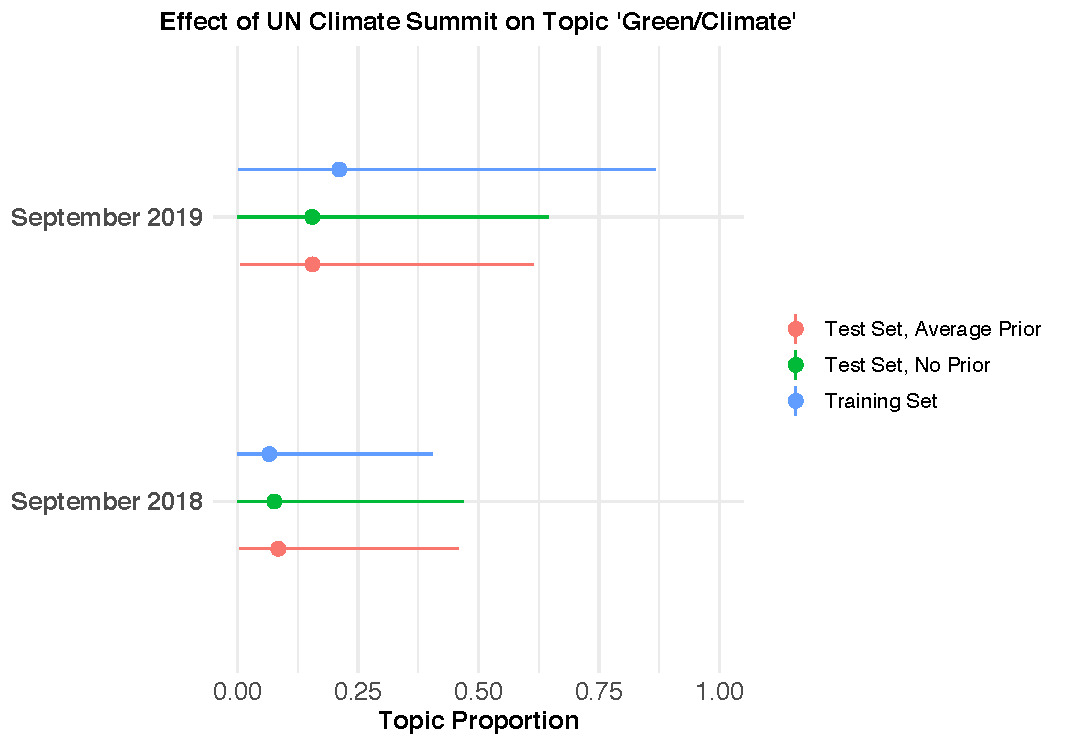
\includegraphics[width=\linewidth]{../plots/4_7/climate_summit_props.pdf}
  \end{subfigure}
  \begin{subfigure}[b]{0.49\linewidth}
    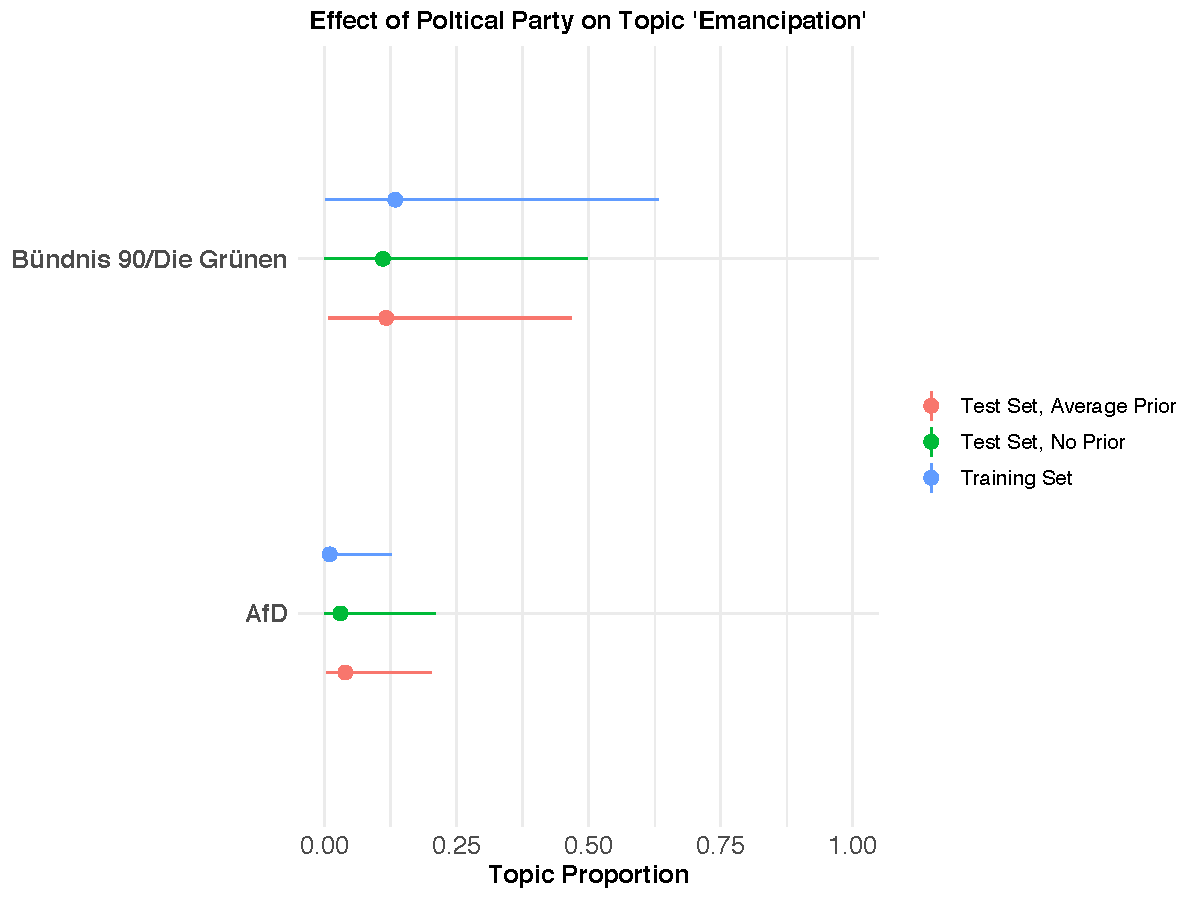
\includegraphics[width=\linewidth]{../plots/4_7/emancipation_props.pdf}
  \end{subfigure}
  \caption{Maximum-a-posteriori (MAP) estimates of topic proportions on training and test data. Points display the mean, lines 2.5\% and 97.5\% credible intervals.}
  \label{fig:causal_inference_props}
\end{figure}

If we want to estimate the treatment effect, we can estimate the average difference of MAP estimates between both groups. Following \cite{egami2018make}, we obtain an estimate of the Average Treatment Effect (ATE) on a data set $\mathcal{D}$ as 
\begin{align}
\widehat{\text{ATE}} = \frac{1}{|\mathcal{D}_{\text{treatment}}|}\sum_{i \in \mathcal{D}_{\text{treatment}}} \hat{\theta}_i - \frac{1}{|\mathcal{D}_{\text{control}}|}\sum_{i \in \mathcal{D}_{\text{control}}} \hat{\theta}_i,
\end{align} 
where $\hat{\theta}_i$ is the MAP estimate for the $i$-th document. \cite{egami2018make} show that, if additional conditions hold, the estimated $\widehat{\text{ATE}}$ on previously unseen test data $\mathcal{D}_{\text{test}}$ is an unbiased estimate of the ATE.

In Figure \ref{fig:causal_inference_ate} we visualize the ATE estimated on training and on test data with different prior specifications (note that this is simply the difference of the means depicted in Figure \ref{fig:causal_inference_props}). The results correspond to our classical idea of overfitting: since the characteristics of each parliamentarian associated with a document have been used to estimate the topic proportions in the first place, when evaluating the effects of these characteristics on topic proportions on the same data, the effect is optimistically biased.

\begin{figure}[h!]
  \centering
  \captionsetup{justification=centering,margin=2cm}
  \begin{subfigure}[b]{0.49\linewidth}
    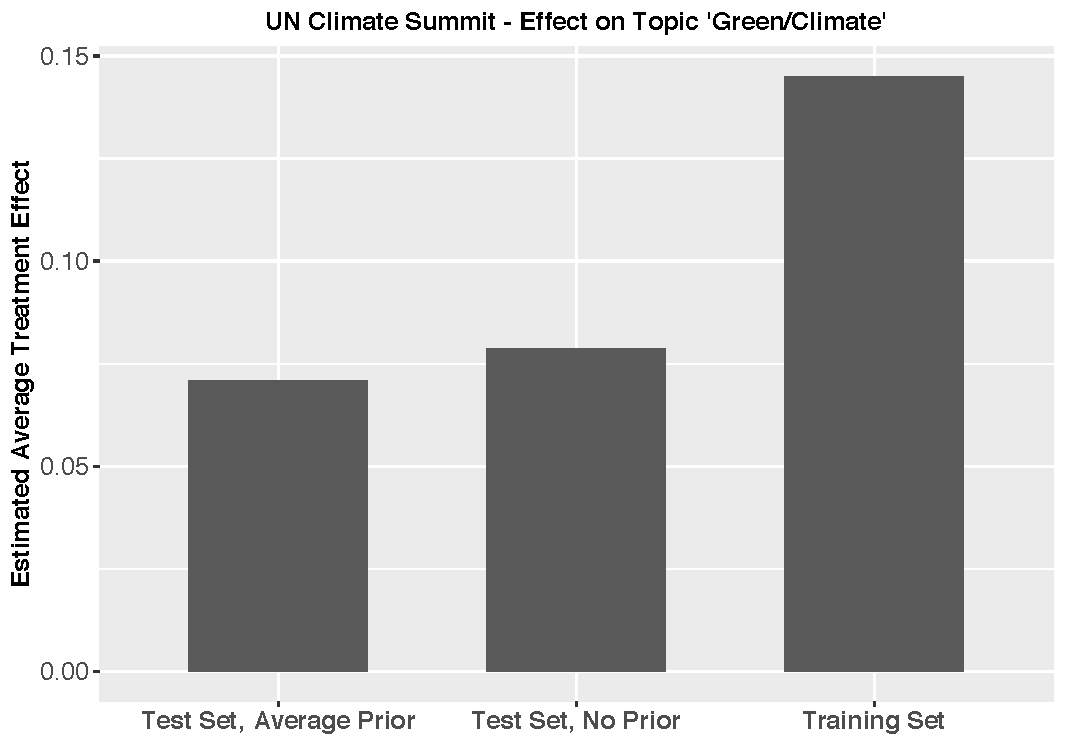
\includegraphics[width=\linewidth]{../plots/4_7/climate_summit_ate.pdf}
  \end{subfigure}
  \begin{subfigure}[b]{0.49\linewidth}
    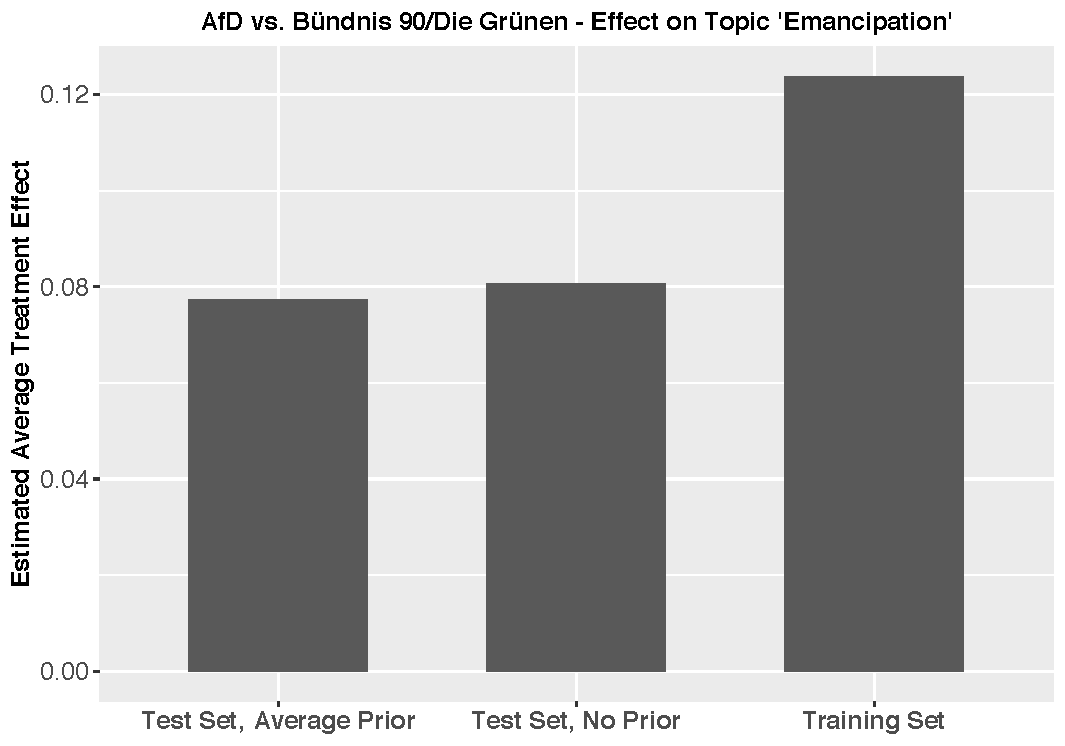
\includegraphics[width=\linewidth]{../plots/4_7/emancipation_ate.pdf}
  \end{subfigure}
  \caption{Estimated Average Treatment Effects (ATE) using training and test data.}
  \label{fig:causal_inference_ate}
\end{figure}

Before we finish this section, we want to remind the reader that there are several general concerns when conducting a causal inference study. For instance, if the treatment group is not a random subsample of the population, but instead assignment to this group is related to the causal effect of interest, the resulting estimator of the treatment effect will suffer a selection bias.